\chapter{Implementation}
\label{chapter:Implementation}

In this chapter, we discuss implementation details of our approach introduced in 
\ref{chapter:Methods}. The first section discusses the creation of a annotated dataset 
for train, separately, the part based detection and the template based algorithm, while 
in the second section, we describe will describe development environment, and  training procedure.

\section{Dataset - Part based model}
In this section, We discuss the details involve in the creation of the dataset for
train the algorithm define in \ref{chapter:Methods}, during the project we acquire
a big amount of data, considering different in daylight light, water properties and
with different fish types, but for this work, and due that the data preparation is 
handwork intensely, we process a specific set of data, in which all the experiment
will be performed, to achieve this goal, a small C++ application was developed.
As introduced in \ref{chapter:Methods} the fish is model using the concept of stickmen, that
mean the each part is define by its coordinates $(x,y)$ and joint through a line.
analysing the fish structure, we create two dataset modelling the fish with 3 and 7 parts, as shown in
figure \ref{fig:anotated1} and \ref{fig:anotated1} respectively.

base on this two created dataset, it is possible then to extrapolate the model linearly,
using a simple matrix multiplication as define in equation \ref{eq:extrapole}, enabling us to 
test our propose algorithm with for example 5, 9, 11 part fish model.


\begin{equation}
 \label{eq:extrapole}
\hat{point}_{m'xn} =\mathtt{A}_{m'xm} \cdot point_{mxn}
\end{equation}

where
 \begin{equation}
\mathtt{A} =
\begin{bmatrix}
a_{11}  & a_{12}  & 0 & \cdots & \cdots & \cdots & \cdots & 0 \\
a_{21}  & a_{22}  & a_{23}  & \ddots & && & \vdots \\
0 & a_{32}  & a_{33} & a_{34}  & \ddots & &  & \vdots \\
\vdots & \ddots & \ddots & \ddots & \ddots & \ddots &  & \vdots \\
\vdots & & \ddots & \ddots & \ddots & \ddots & \ddots& \vdots\\
\vdots  &  & & \ddots & a_{(m'-2)(m-3)}  & a_{(m'-2)(m-2)}  &  a_{(m'-2)(m-1)}  & 0\\
\vdots  &  & & & \ddots & a_{(m'-1)(m-2)}  & a_{(m'-1)(m_1)}  &  a_{(m'-1)m}\\
0 & \cdots &  \cdots & \cdots & \cdots & 0 & a_{m'(m-1)} & a_{m'm}  \\
\end{bmatrix}
 \end{equation}


\begin{figure}
\begin{adjustwidth}{-1in}{-1in} 
\label{fig:anotated1}
\centering     %%% not \center
\subfigure[]{\label{fig:a}\includegraphics[width=70mm]{anotated/3/data_st11_led0_0021}}
\subfigure[]{\label{fig:a}\includegraphics[width=70mm]{anotated/3/data_st11_led0_0023}}
\subfigure[]{\label{fig:a}\includegraphics[width=70mm]{anotated/3/data_st11_led0_0025}}
\subfigure[]{\label{fig:a}\includegraphics[width=70mm]{anotated/3/data_st11_led0_0027}}
\caption{This illustrates the annotated fish in a 3 Part model}
\end{adjustwidth}
\end{figure}

\begin{figure}
\begin{adjustwidth}{-1in}{-1in} 
\label{fig:anotated1}
\centering     %%% not \center
\subfigure[]{\label{fig:a}\includegraphics[width=70mm]{anotated/5/data_st11_led0_0021}}
\subfigure[]{\label{fig:a}\includegraphics[width=70mm]{anotated/5/data_st11_led0_0023}}
\subfigure[]{\label{fig:a}\includegraphics[width=70mm]{anotated/5/data_st11_led0_0025}}
\subfigure[]{\label{fig:a}\includegraphics[width=70mm]{anotated/5/data_st11_led0_0027}}
\caption{This illustrates the annotated fish in a 7 Part model}
\end{adjustwidth}
\end{figure}

now as a example, to extrapolate from a 3 parts model to a 5 parts model, the matrix
should look like this:


\begin{equation}
\hat{point}_{9x2} =\mathtt{A}_{9x3} \cdot point_{3x2}
\end{equation}

where
 \begin{equation}
 \label{eq:extrapole}
\mathtt{A} =
\begin{bmatrix}
1  & 0 & 0 & 0 & 0 & 0 & 0 \\
\frac{1}{2} & \frac{1}{2}  & 0 & 0 & 0 & 0 & 0 \\
0 & 1  & 0 & 0 & 0 & 0 & 0  \\
0 & \frac{1}{2} & \frac{1}{2} & 0 & 0 & 0 & 0 \\
0  & 0 & 1 & 0 & 0 & 0 & 0  \\
0  & 0 & 0 & 1 & 0 & 0 & 0  \\
0  & 0 & 0 & 0 & 1 & 0 & 0 \\
0  & 0 & 0 & 0 & 0 & 1 & 0 \\
0  & 0 & 0 & 0 & 0 & 0 & 1  \\
\end{bmatrix}
 \end{equation}

and each $\frac{1}{2}$ represent the middle point between the two original annotated
points.

\begin{figure}
\begin{adjustwidth}{-1in}{-1in} 
\label{fig:anotated1}
\centering     %%% not \center
\subfigure[]{\label{fig:a}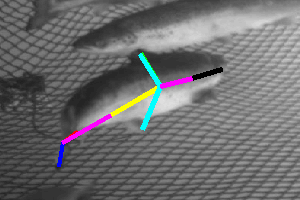
\includegraphics[width=70mm]{anotated/9_extra/extra_9_01}}
\subfigure[]{\label{fig:a}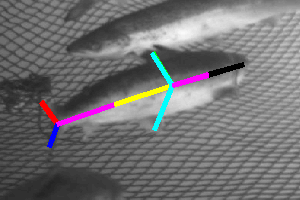
\includegraphics[width=70mm]{anotated/9_extra/extra_9_02}}
\caption{This illustrates the annotated fish in a 9 Part model, where is clearly visible
the new points define in the middle point of the existent parts.}
\end{adjustwidth}
\end{figure}

 \section{Dataset - Template based model based model}
 In this section, We discuss the details involve in the creation of the dataset for
 train the algorithm define in \ref{sec:templatedbased}, as said before for the template 
 matching algorithm, we propose a different way to generate the proper templates, 
 we have template for the Head and Tail, and we train two different linemod detector,
 one for each part, in the figures \ref{fig:head_1}, \ref{fig:head_2}, \ref{fig:tail_1} and
 \ref{fig:tail_2} is show the head of the fish and his corresponding annotated mask, 
 the same can be appreciated for the tail of the fish. the task of create the dataset
 for this project, was one of the most time consuming part, due to, as mentioned before, 
 the nature of the linemod algorithm is to be apply on rigid object, and we are approximating to this
 assumption by dividing the fish in two part, expecting that the deformation suffer from the
 fish, can be isolate into those two part.

\begin{figure}
\begin{adjustwidth}{-1in}{-1in} 
\label{fig:head_1}
\centering     %%% not \center
\subfigure[]{\label{fig:a}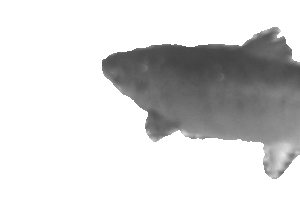
\includegraphics[width=40mm]{anotated/linemod/head/data_st11_led0_0219-4}}
\subfigure[]{\label{fig:a}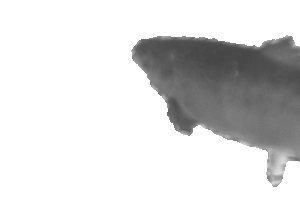
\includegraphics[width=40mm]{anotated/linemod/head/data_st11_led0_0221-4}}
\subfigure[]{\label{fig:a}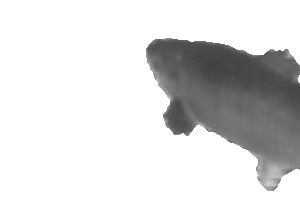
\includegraphics[width=40mm]{anotated/linemod/head/data_st11_led0_0223-4}}
\subfigure[]{\label{fig:a}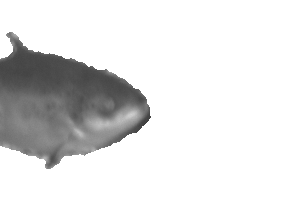
\includegraphics[width=40mm]{anotated/linemod/head/data_st11_led0_0227-4}}
\subfigure[]{\label{fig:a}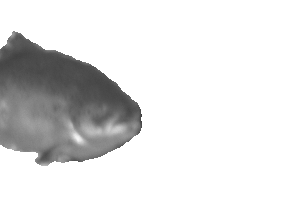
\includegraphics[width=40mm]{anotated/linemod/head/data_st11_led0_0229-4}}
\subfigure[]{\label{fig:a}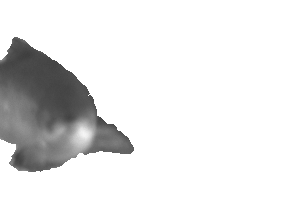
\includegraphics[width=40mm]{anotated/linemod/head/data_st11_led0_0231-4}}
\subfigure[]{\label{fig:a}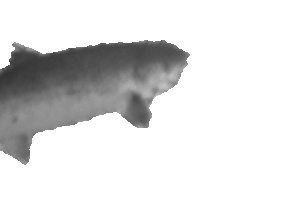
\includegraphics[width=40mm]{anotated/linemod/head/data_st11_led0_0233-4}}
\subfigure[]{\label{fig:a}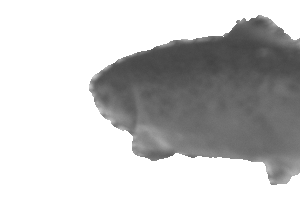
\includegraphics[width=40mm]{anotated/linemod/head/data_st11_led0_0235-4}}
\caption{This illustrates the annotated fish head, need it for train the linemod detector}
\end{adjustwidth}
\end{figure}

\begin{figure}
\begin{adjustwidth}{-1in}{-1in} 
\label{fig:head_2}
\centering     %%% not \center
\subfigure[]{\label{fig:a}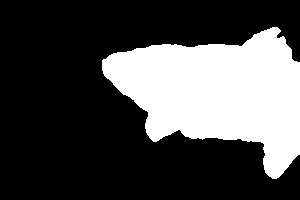
\includegraphics[width=40mm]{anotated/linemod/head/data_st11_led0_0219-3}}
\subfigure[]{\label{fig:a}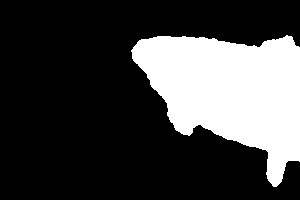
\includegraphics[width=40mm]{anotated/linemod/head/data_st11_led0_0221-3}}
\subfigure[]{\label{fig:a}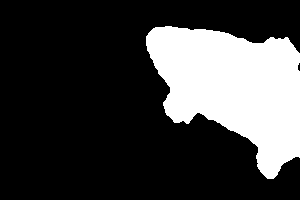
\includegraphics[width=40mm]{anotated/linemod/head/data_st11_led0_0223-3}}
\subfigure[]{\label{fig:a}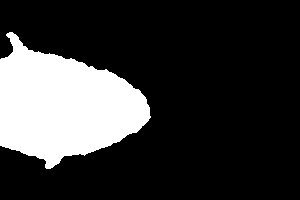
\includegraphics[width=40mm]{anotated/linemod/head/data_st11_led0_0227-3}}
\subfigure[]{\label{fig:a}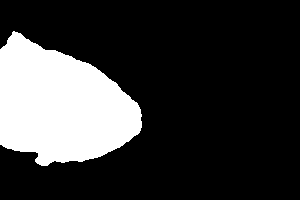
\includegraphics[width=40mm]{anotated/linemod/head/data_st11_led0_0229-3}}
\subfigure[]{\label{fig:a}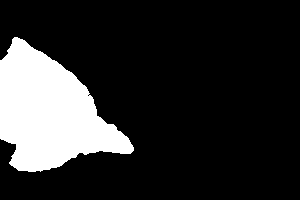
\includegraphics[width=40mm]{anotated/linemod/head/data_st11_led0_0231-3}}
\subfigure[]{\label{fig:a}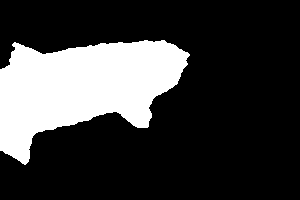
\includegraphics[width=40mm]{anotated/linemod/head/data_st11_led0_0233-3}}
\subfigure[]{\label{fig:a}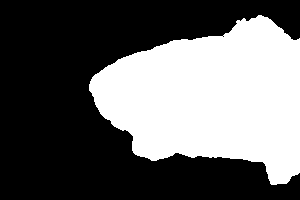
\includegraphics[width=40mm]{anotated/linemod/head/data_st11_led0_0235-3}}
\caption{This illustrates the annotated mask fish head, need it for train the linemod detector}
\end{adjustwidth}
\end{figure}

\begin{figure}
\begin{adjustwidth}{-1in}{-1in} 
\label{fig:tail_1}
\centering     %%% not \center
\subfigure[]{\label{fig:a}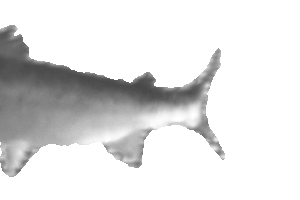
\includegraphics[width=40mm]{anotated/linemod/tail/data_st11_led0_0219-6}}
\subfigure[]{\label{fig:a}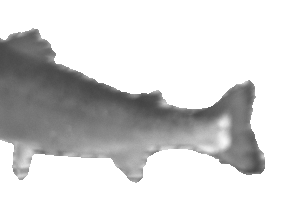
\includegraphics[width=40mm]{anotated/linemod/tail/data_st11_led0_0221-6}}
\subfigure[]{\label{fig:a}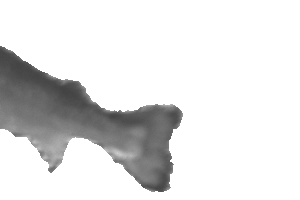
\includegraphics[width=40mm]{anotated/linemod/tail/data_st11_led0_0223-6}}
\subfigure[]{\label{fig:a}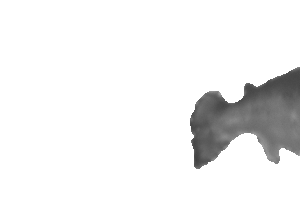
\includegraphics[width=40mm]{anotated/linemod/tail/data_st11_led0_0227-6}}
\subfigure[]{\label{fig:a}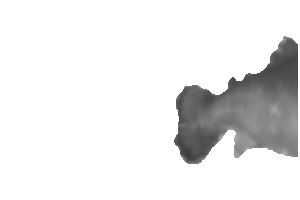
\includegraphics[width=40mm]{anotated/linemod/tail/data_st11_led0_0229-6}}
\subfigure[]{\label{fig:a}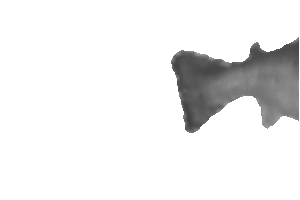
\includegraphics[width=40mm]{anotated/linemod/tail/data_st11_led0_0231-6}}
\subfigure[]{\label{fig:a}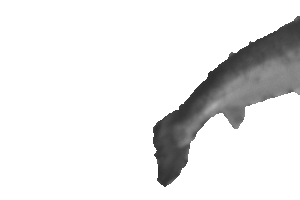
\includegraphics[width=40mm]{anotated/linemod/tail/data_st11_led0_0233-6}}
\subfigure[]{\label{fig:a}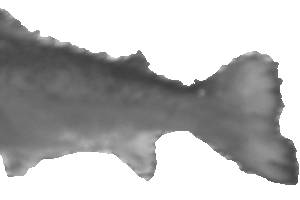
\includegraphics[width=40mm]{anotated/linemod/tail/data_st11_led0_0235-6}}
\caption{This illustrates the annotated fish tail, need it for train the linemod detector}
\end{adjustwidth}
\end{figure}

\begin{figure}
\begin{adjustwidth}{-1in}{-1in} 
\label{fig:tail_2}
\centering     %%% not \center
\subfigure[]{\label{fig:a}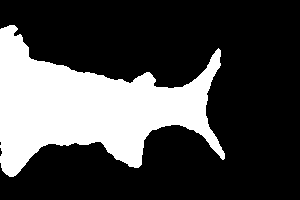
\includegraphics[width=40mm]{anotated/linemod/tail/data_st11_led0_0219-5}}
\subfigure[]{\label{fig:a}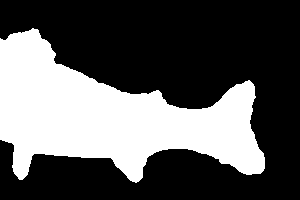
\includegraphics[width=40mm]{anotated/linemod/tail/data_st11_led0_0221-5}}
\subfigure[]{\label{fig:a}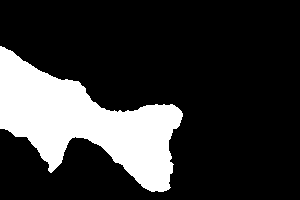
\includegraphics[width=40mm]{anotated/linemod/tail/data_st11_led0_0223-5}}
\subfigure[]{\label{fig:a}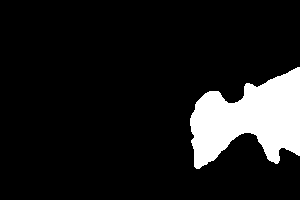
\includegraphics[width=40mm]{anotated/linemod/tail/data_st11_led0_0227-5}}
\subfigure[]{\label{fig:a}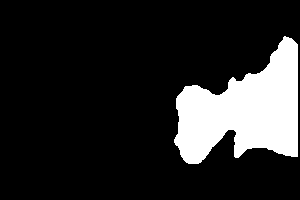
\includegraphics[width=40mm]{anotated/linemod/tail/data_st11_led0_0229-5}}
\subfigure[]{\label{fig:a}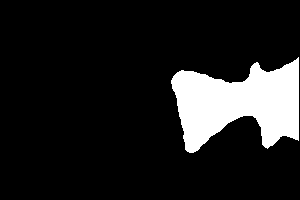
\includegraphics[width=40mm]{anotated/linemod/tail/data_st11_led0_0231-5}}
\subfigure[]{\label{fig:a}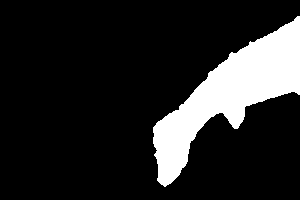
\includegraphics[width=40mm]{anotated/linemod/tail/data_st11_led0_0233-5}}
\subfigure[]{\label{fig:a}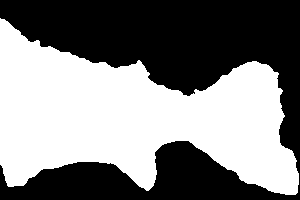
\includegraphics[width=40mm]{anotated/linemod/tail/data_st11_led0_0235-5}}
\caption{This illustrates the annotated mask fish tail, need it for train the linemod detector}
\end{adjustwidth}
\end{figure}

\section{Software implementation}
In this section, we will discuss implementation details involve in this work,
relate with tools and algorithm used.

\begin{itemize}
\item \textit{Part Based algorithm } from section \ref{sec:partbased} was implemented in 
MATLAB, and the code can be found on the author website (\url{http://www.ics.uci.edu/~dramanan/}), 
this code was modified to process our specific dataset. and considering the highly expensive 
computational require by this algorithm, the deployment
of it was perform in the \textit{Linux-Cluster} from our University. which consists of several
 segments with different types of interconnect and different sizes of shared memory. 
 All systems have a (virtual) 64 bit address space.
	\begin{itemize}	
	\item \textit{Learning} our learning process starts by loading the 2D intensity 
	image from the annotated dataset, and randomly sampling the images and pixels. 
	this samples are used as input as define for equation \ref{eq:learning}. This
	process is repeated until all the constraint are fulfilled, and the learned parameter 
	are save as a MAT file (Microsoft Access Table Shortcut file).
	\item \textit{Prediction and Runtime} Using a different dataset, we start loading
	the trained model, given a 2D image the algorithm output a set of candidates, 
	define by its bounding boxes, to be able to combine the template based algorithm, 
	which is implemented in C++ and using opencv, and this one, we used a implementation
	of the algorithm ported to C++ and is available in 
	(\url{https://github.com/wg-perception/PartsBasedDetector}).
	\end{itemize}
\item{Template based algorithm } from section \ref{sec:templatebased} was implemented in C++ 
using the computer vision library OpenCV.
	\begin{itemize}
	\item \textit{Learning} our learning process starts by loading the  2D intensity 
	image from the annotated dataset, recall that two different detector are trained, 
	one for the head and other for the tail, and Adding the template to the database as 
	mention in \citet{Hinterstoisser2012} and describe in section \ref{sec:templatebase}. 
	This process in repeated to our entire dataset and learned parameter are save as a
	binary file.
	\item \textit{Detection and Runtime} Using a different dataset, we start loading
	the trained model, given a 2D image with its corresponding labeled mask, coming from
	the part based algorithm, the algorithm output a set of detect contour for the head
	and tail of the fish, Initially, the output was not as good as expected, due to
	the nature of the training data, but then, we include a verification test to ensure 
	that the set of head-tail contour is geometrically feasible, as explained in section
	\ref{sec:proposeworkflow}
	\end{itemize}
\end{itemize}
